\documentclass[tikz,border=8pt]{standalone}
\usepackage{amsmath}
\usepackage{amssymb}
\usepackage{tikz}
\usetikzlibrary{arrows.meta,calc,decorations.pathreplacing,patterns,shapes.geometric,positioning,shadings}

\begin{document}
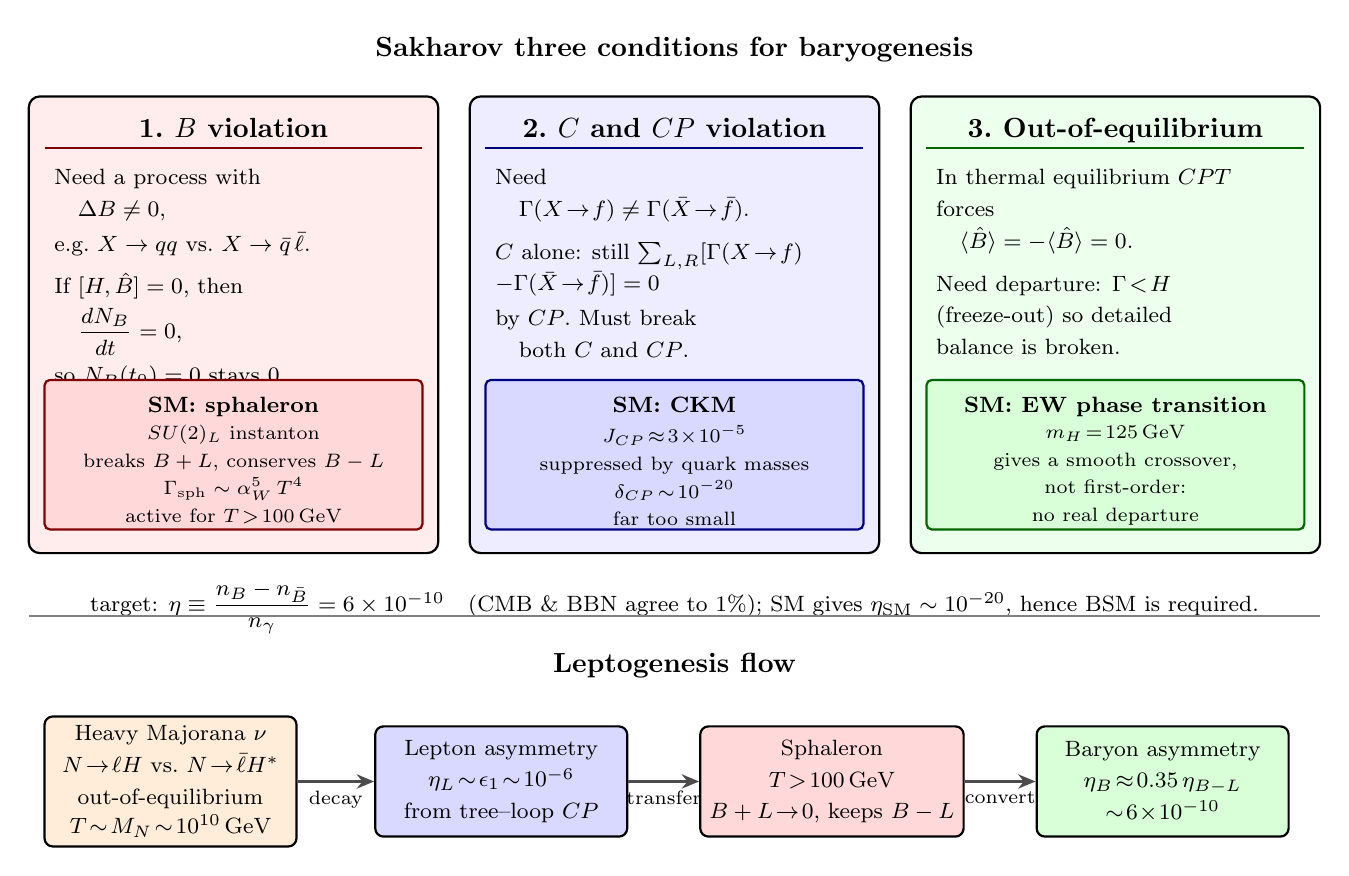
\begin{tikzpicture}[>={Stealth[length=2.2mm,width=1.8mm]},font=\small]

%================ TOP TITLE ================
\node[font=\bfseries] at (8,7.6) {Sakharov three conditions for baryogenesis};

%================ COLUMN 1: B violation ================
\begin{scope}[shift={(0,0)}]
  % box
  \draw[thick,rounded corners=4pt,fill=red!7] (-0.2,1.2) rectangle (5.0,7.0);
  % header
  \node[font=\bfseries,anchor=north] at (2.4,6.85) {1.\ $B$ violation};
  \draw[thick,red!50!black] (0.0,6.35) -- (4.8,6.35);

  % content
  \node[anchor=north west,align=left,font=\footnotesize] at (0.0,6.2) {%
    Need a process with\\[2pt]
    \quad $\Delta B \neq 0$,\\[3pt]
    e.g.\ $X \to qq$ vs.\ $X \to \bar q\,\bar\ell$.\\[6pt]
    If $[H,\hat B]=0$, then\\[2pt]
    \quad $\dfrac{dN_B}{dt}=0$,\\[3pt]
    so $N_B(t_0)=0$ stays $0$.};

  % SM realization box
  \draw[thick,red!50!black,rounded corners=2pt,fill=red!15] (0.0,1.5) rectangle (4.8,3.4);
  \node[anchor=north,font=\footnotesize\bfseries] at (2.4,3.3) {SM: sphaleron};
  \node[anchor=north,align=center,font=\scriptsize] at (2.4,2.95) {%
    $SU(2)_L$ instanton\\[2pt]
    breaks $B+L$, conserves $B-L$\\[2pt]
    $\Gamma_{\text{sph}}\sim\alpha_W^5\,T^4$\\[2pt]
    active for $T\!>\!100\,\text{GeV}$};
\end{scope}

%================ COLUMN 2: C+CP violation ================
\begin{scope}[shift={(5.6,0)}]
  \draw[thick,rounded corners=4pt,fill=blue!7] (-0.2,1.2) rectangle (5.0,7.0);
  \node[font=\bfseries,anchor=north] at (2.4,6.85) {2.\ $C$ and $CP$ violation};
  \draw[thick,blue!50!black] (0.0,6.35) -- (4.8,6.35);

  \node[anchor=north west,align=left,font=\footnotesize] at (0.0,6.2) {%
    Need\\[2pt]
    \quad $\Gamma(X\!\to\! f)\neq\Gamma(\bar X\!\to\!\bar f)$.\\[6pt]
    $C$ alone: still
    $\sum_{L,R}[\Gamma(X\!\to\! f)$\\
    $-\Gamma(\bar X\!\to\!\bar f)]=0$\\[3pt]
    by $CP$.\ Must break\\[2pt]
    \quad both $C$ and $CP$.};

  \draw[thick,blue!50!black,rounded corners=2pt,fill=blue!15] (0.0,1.5) rectangle (4.8,3.4);
  \node[anchor=north,font=\footnotesize\bfseries] at (2.4,3.3) {SM: CKM};
  \node[anchor=north,align=center,font=\scriptsize] at (2.4,2.95) {%
    $J_{CP}\!\approx\!3\!\times\!10^{-5}$\\[2pt]
    suppressed by quark masses\\[2pt]
    $\delta_{CP}\!\sim\!10^{-20}$\\[2pt]
    far too small};
\end{scope}

%================ COLUMN 3: out-of-equilibrium ================
\begin{scope}[shift={(11.2,0)}]
  \draw[thick,rounded corners=4pt,fill=green!7] (-0.2,1.2) rectangle (5.0,7.0);
  \node[font=\bfseries,anchor=north] at (2.4,6.85) {3.\ Out-of-equilibrium};
  \draw[thick,green!40!black] (0.0,6.35) -- (4.8,6.35);

  \node[anchor=north west,align=left,font=\footnotesize] at (0.0,6.2) {%
    In thermal equilibrium $CPT$\\[2pt]
    forces\\[2pt]
    \quad $\langle\hat B\rangle=-\langle\hat B\rangle=0$.\\[6pt]
    Need departure: $\Gamma\!<\!H$\\[2pt]
    (freeze-out) so detailed\\[2pt]
    balance is broken.};

  \draw[thick,green!40!black,rounded corners=2pt,fill=green!15] (0.0,1.5) rectangle (4.8,3.4);
  \node[anchor=north,font=\footnotesize\bfseries] at (2.4,3.3) {SM: EW phase transition};
  \node[anchor=north,align=center,font=\scriptsize] at (2.4,2.95) {%
    $m_H\!=\!125\,\text{GeV}$\\[2pt]
    gives a smooth crossover,\\[2pt]
    not first-order:\\[2pt]
    no real departure};
\end{scope}

%================ TARGET BAR ================
\node[font=\footnotesize,anchor=north] at (8,0.95)
  {target: $\eta\equiv\dfrac{n_B-n_{\bar B}}{n_\gamma}=6\times 10^{-10}$\quad
   (CMB \& BBN agree to $1\%$); SM gives $\eta_{\text{SM}}\sim 10^{-20}$, hence BSM is required.};

\draw[thick,black!50] (-0.2,0.4) -- (16.2,0.4);

%================ BOTTOM FLOW: leptogenesis ================
\node[font=\bfseries,anchor=north] at (8,0.05) {Leptogenesis flow};

% Step 1: heavy nu decay
\node[draw,thick,rounded corners=3pt,fill=orange!15,align=center,font=\footnotesize,
      minimum width=3.2cm,minimum height=1.4cm] (S1) at (1.6,-1.7) {%
  Heavy Majorana $\nu$\\[2pt]
  $N\!\to\!\ell H$ vs.\ $N\!\to\!\bar\ell H^*$\\[2pt]
  out-of-equilibrium\\[1pt]
  $T\!\sim\! M_N\!\sim\! 10^{10}\,\text{GeV}$};

% Step 2: L asymmetry
\node[draw,thick,rounded corners=3pt,fill=blue!15,align=center,font=\footnotesize,
      minimum width=3.2cm,minimum height=1.4cm] (S2) at (5.8,-1.7) {%
  Lepton asymmetry\\[2pt]
  $\eta_L\!\sim\!\epsilon_1\!\sim\! 10^{-6}$\\[2pt]
  from tree--loop $CP$};

% Step 3: sphaleron
\node[draw,thick,rounded corners=3pt,fill=red!15,align=center,font=\footnotesize,
      minimum width=3.2cm,minimum height=1.4cm] (S3) at (10.0,-1.7) {%
  Sphaleron\\[2pt]
  $T\!>\!100\,\text{GeV}$\\[2pt]
  $B+L\!\to\! 0$, keeps $B-L$};

% Step 4: B asymmetry
\node[draw,thick,rounded corners=3pt,fill=green!15,align=center,font=\footnotesize,
      minimum width=3.2cm,minimum height=1.4cm] (S4) at (14.2,-1.7) {%
  Baryon asymmetry\\[2pt]
  $\eta_B\!\approx\! 0.35\,\eta_{B-L}$\\[2pt]
  $\sim\! 6\!\times\!10^{-10}$};

% Arrows between
\draw[->,very thick,black!70] (S1.east) -- (S2.west);
\draw[->,very thick,black!70] (S2.east) -- (S3.west);
\draw[->,very thick,black!70] (S3.east) -- (S4.west);

% Decorations: annotations under arrows
\node[font=\scriptsize,anchor=north] at ($(S1.east)!0.5!(S2.west)+(0,0.0)$) {decay};
\node[font=\scriptsize,anchor=north] at ($(S2.east)!0.5!(S3.west)+(0,0.0)$) {transfer};
\node[font=\scriptsize,anchor=north] at ($(S3.east)!0.5!(S4.west)+(0,0.0)$) {convert};

\end{tikzpicture}
\end{document}
